\section{Annisa Fathoroni/1164067}
\subsection{Teori}
\subsubsection{Soal No. 1}
Kenapa file teks harus dilakukan tokenizer, dilengkapi dengan ilustrasi atau gambar.

Karena tokenizer ini berfungsi untuk mengkonversi teks menjadi urutan integer indeks kata atau vektor binary, word count atau tf-idf. Text harus dilakukan tokenizer agar dapat dirubah menjadi vektor. Dari perubahan ke vektor tersebut maka data/textnya dapat dibaca oleh komputer (terkomputerisasi).

\begin{itemize}
\item Ilustrasi Gambar:

\begin{figure}[!hbtp]
\centering
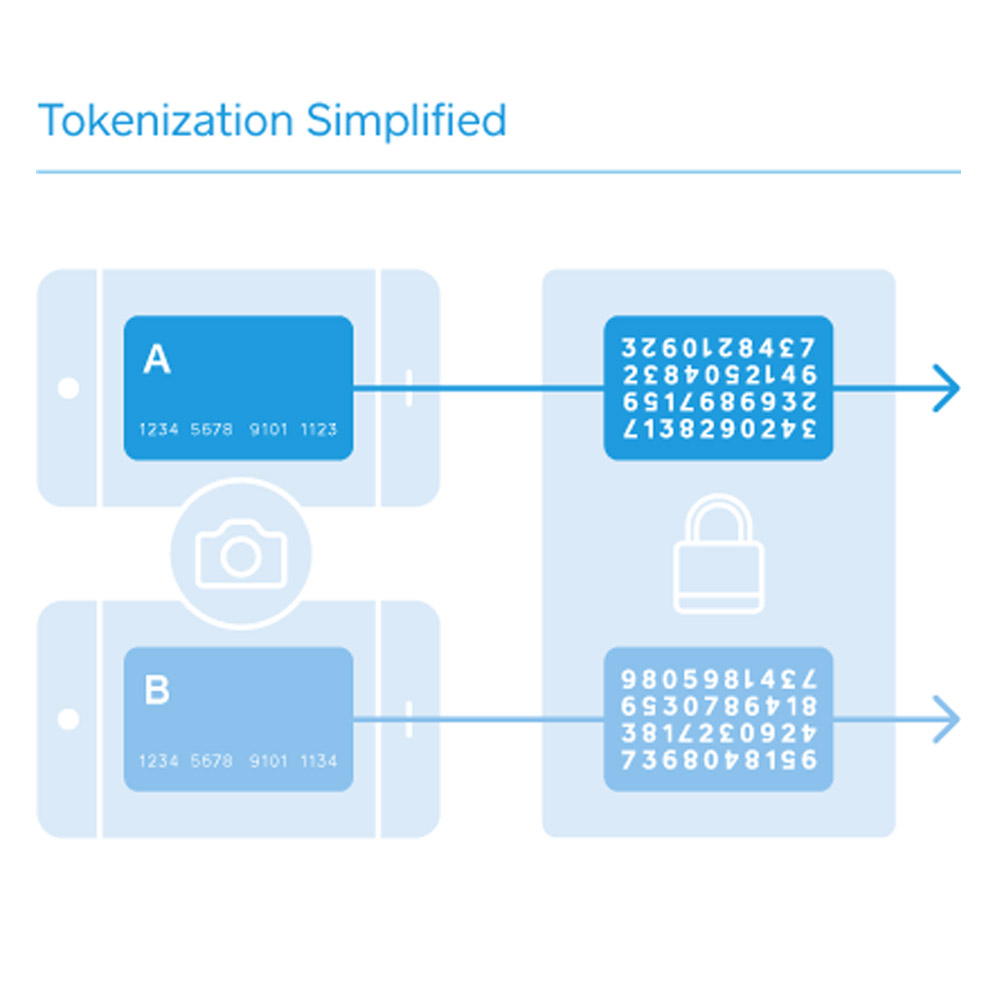
\includegraphics[scale=0.2]{figures/Chapter 7/1164067/Teori/Chapter7AnnisaFathoroni1.jpg}
\caption{Tokenizer - Annisa Fathoroni}
\label{Tokenizer - Annisa Fathoroni}
\end{figure}

\end{itemize}

\subsubsection{Soal No. 2}
Konsep dasar K Fold Cross Validation pada dataset komentar Youtube, dilengkapi dengan ilustrasi atau gambar.

\begin{itemize}
\item Ilustrasi Gambar:

\begin{figure}[!hbtp]
\centering
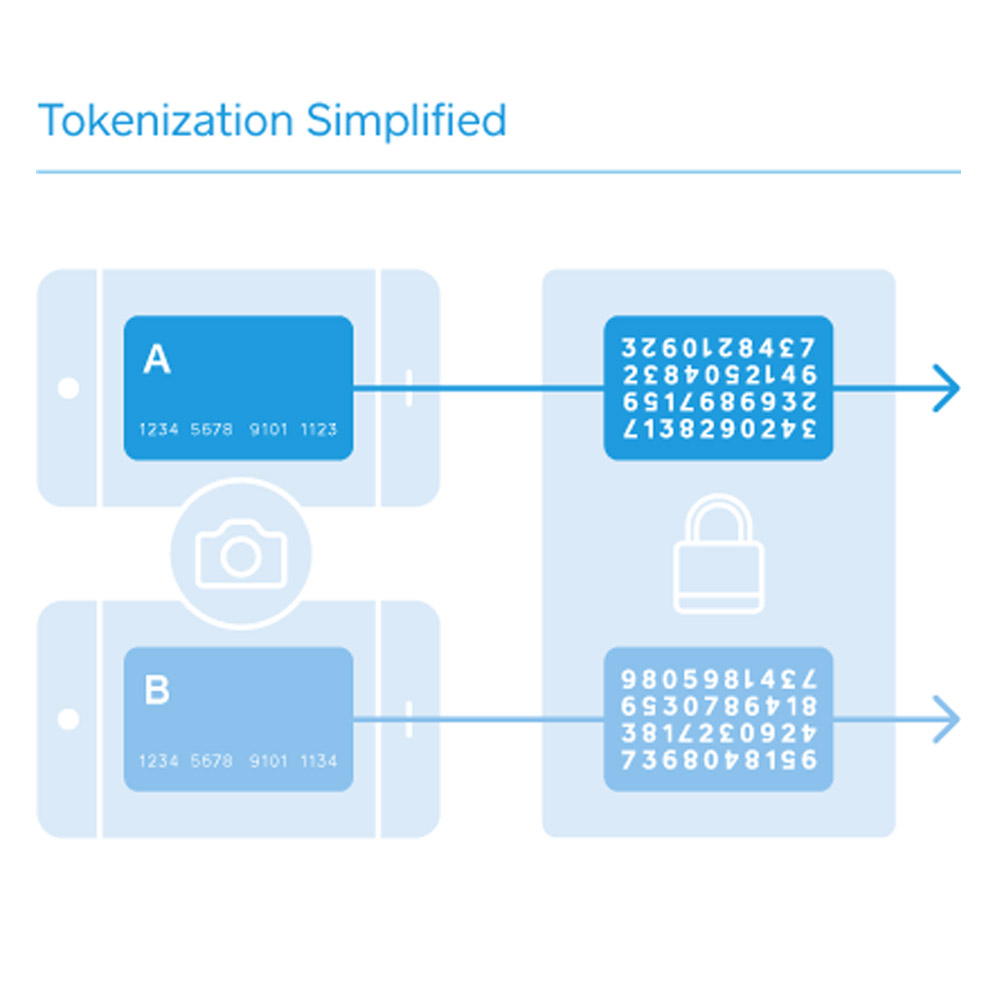
\includegraphics[scale=0.4]{figures/Chapter 7/1164067/Teori/Chapter7AnnisaFathoroni1.jpg}
\caption{Konsep dasar K Fold Cross Validation - Annisa Fathoroni}
\label{Konsep dasar K Fold Cross Validation - Annisa Fathoroni}
\end{figure}

\end{itemize}

\subsubsection{Soal No. 3}
Maksud kode program for train dan test in splits, dilengkapi dengan ilustrasi atau gambar.
\begin{itemize}
    \item Ilustrasi Gambar :
\hfill \break
    \begin{figure}[!hbtp]
    \centering
    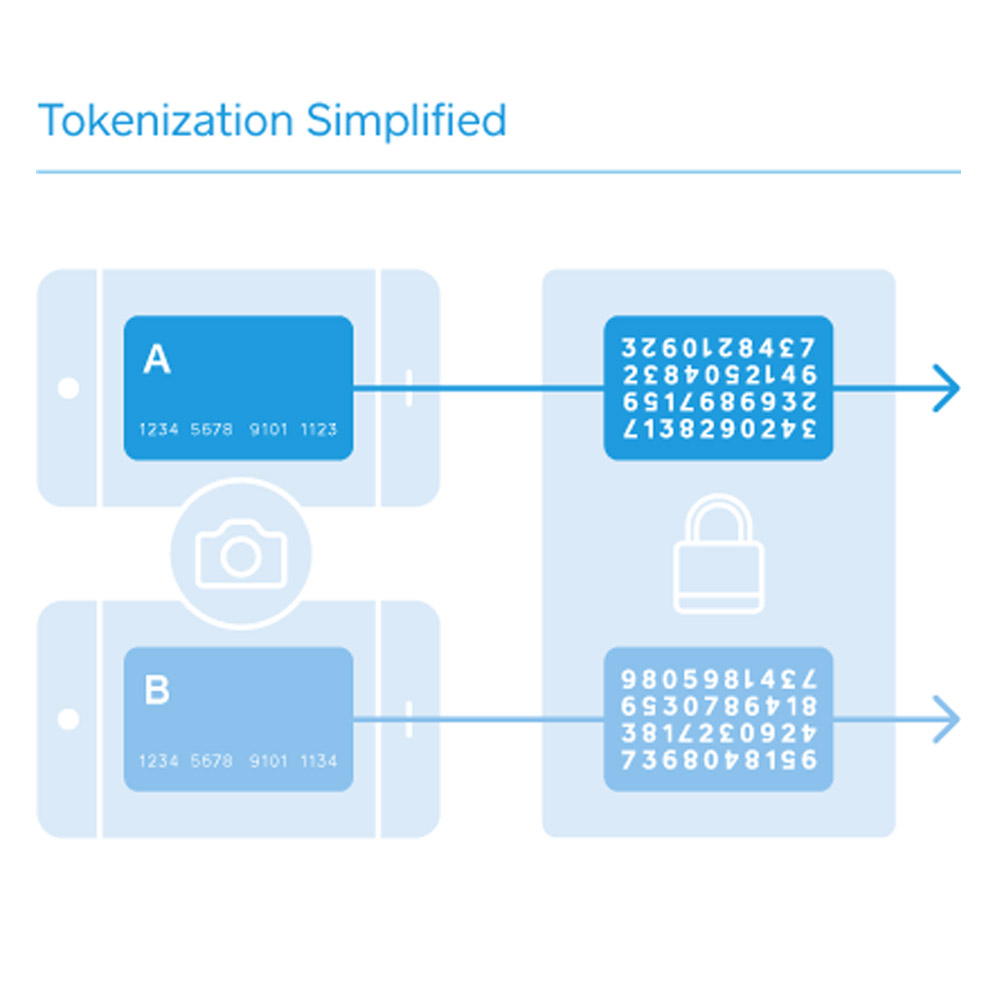
\includegraphics[scale=0.4]{figures/Chapter 7/1164067/Teori/Chapter7AnnisaFathoroni1.jpg}
    \caption{Train - Annisa Fathoroni}
    \label{Train - Annisa Fathoroni}
    \end{figure}

\hfill \break
    \begin{figure}[!hbtp]
    \centering
    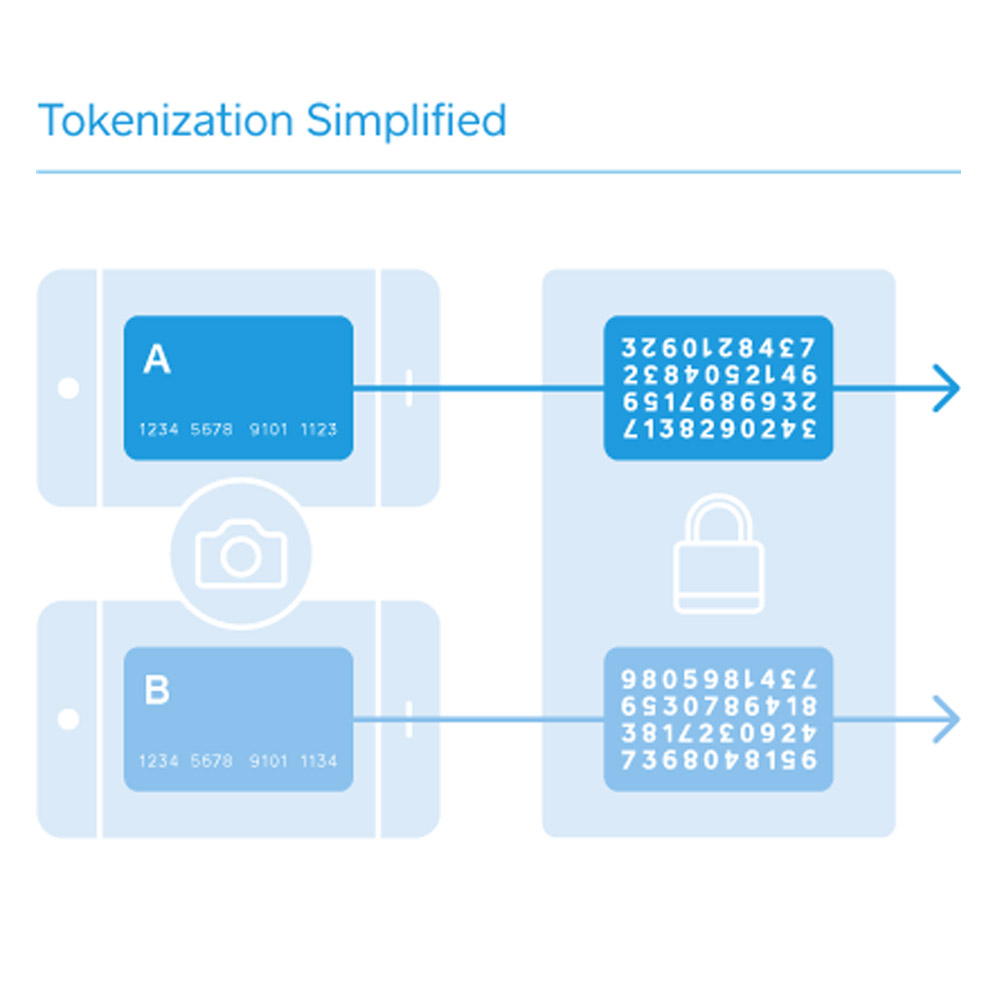
\includegraphics[scale=0.4]{figures/Chapter 7/1164067/Teori/Chapter7AnnisaFathoroni1.jpg}
    \caption{Test in splits - Annisa Fathoroni}
    \label{Test in splits - Annisa Fathoroni}
    \end{figure}

\end{itemize}

\subsubsection{Soal No. 4}
Maksud kode program train content = d[’CONTENT’].iloc[train idx] dan test content = d[’CONTENT’].iloc[test idx], dilengkapi dengan ilustrasi atau gambar.

\begin{itemize}
    \item Ilustrasi Gambar:

    \begin{figure}[!hbtp]
    \centering
    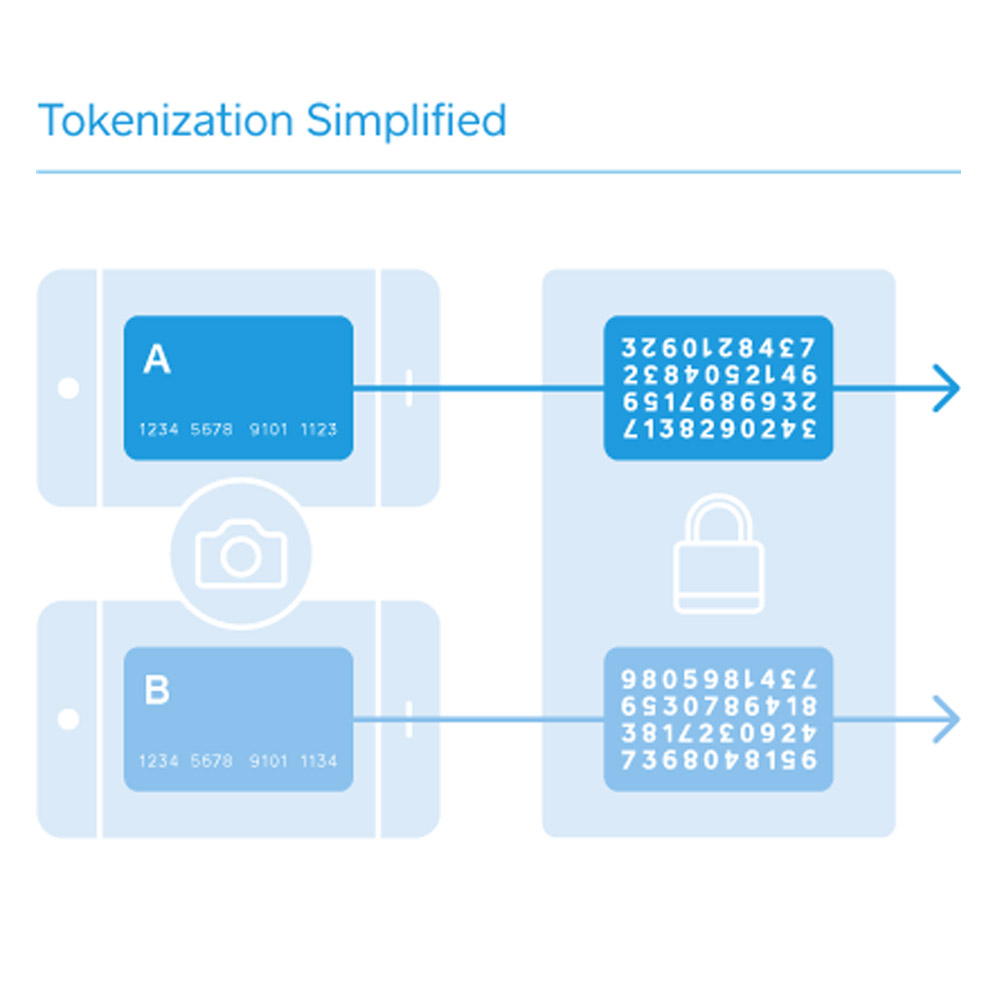
\includegraphics[scale=0.4]{figures/Chapter 7/1164067/Teori/Chapter7AnnisaFathoroni1.jpg}
    \caption{Train content - Annisa Fathoroni}
    \label{Train content - Annisa Fathoroni}
    \end{figure}
\end{itemize}

\subsubsection{Soal No. 5}
Maksud dari fungsi Chapter7AnnisaFathoroni1.jpg = Tokenizer(num words=2000) dan tokenizer.fit on texts(train content), dilengkapi dengan ilustrasi atau gambar.

\begin{itemize}
    \item Ilustrasi Gambar :

    \begin{figure}[!hbtp]
    \centering
    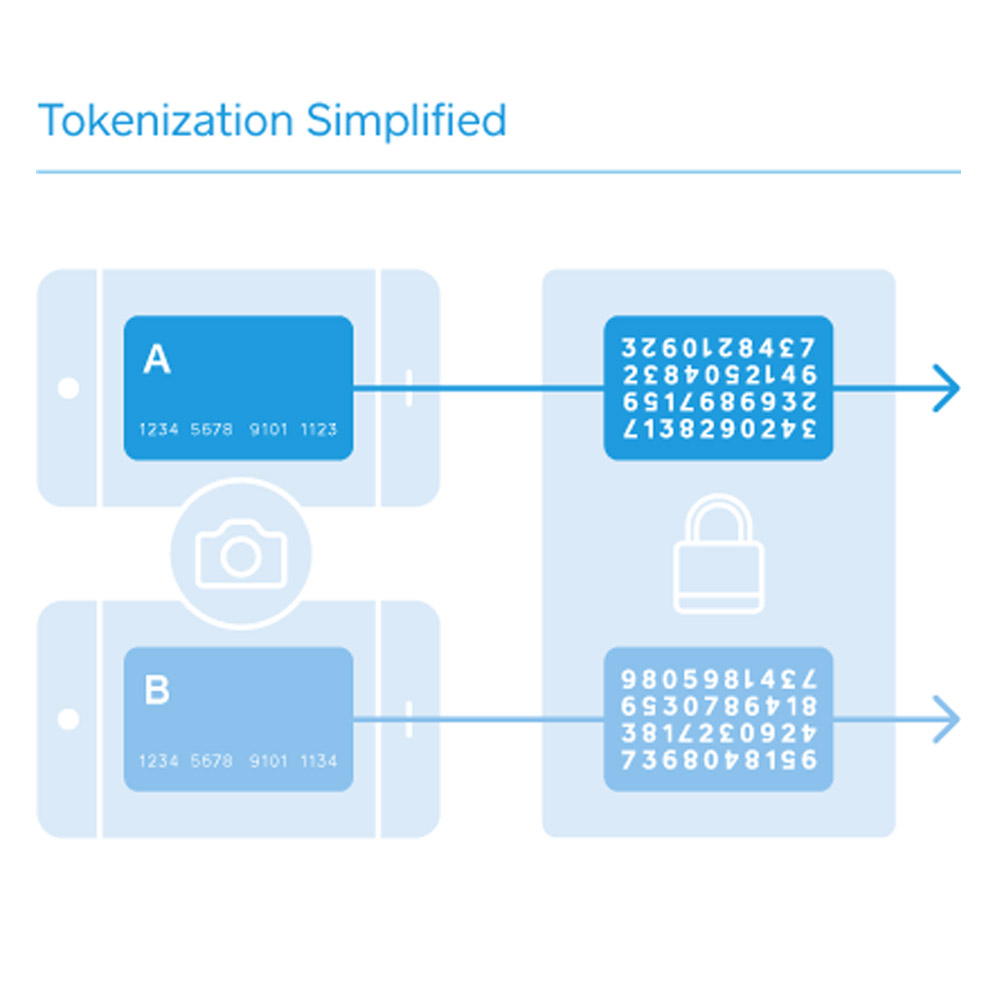
\includegraphics[scale=0.4]{figures/Chapter 7/1164067/Teori/Chapter7AnnisaFathoroni1.jpg}
    \caption{Tokenizer - Annisa Fathoroni}
    \label{Tokenizer - Annisa Fathoroni}
    \end{figure}
\end{itemize}

\subsubsection{Soal No. 6}
Maksud dari fungsi d train inputs = tokenizer.texts to matrix(train content, mode=’tfidf ’) dan d test inputs = tokenizer.texts to matrix(test content, mode=’tfidf ’), dilengkapi dengan ilustrasi atau gambar.

\begin{itemize}
\item Ilustrasi Gambar:

    \begin{figure}[!hbtp]
    \centering
    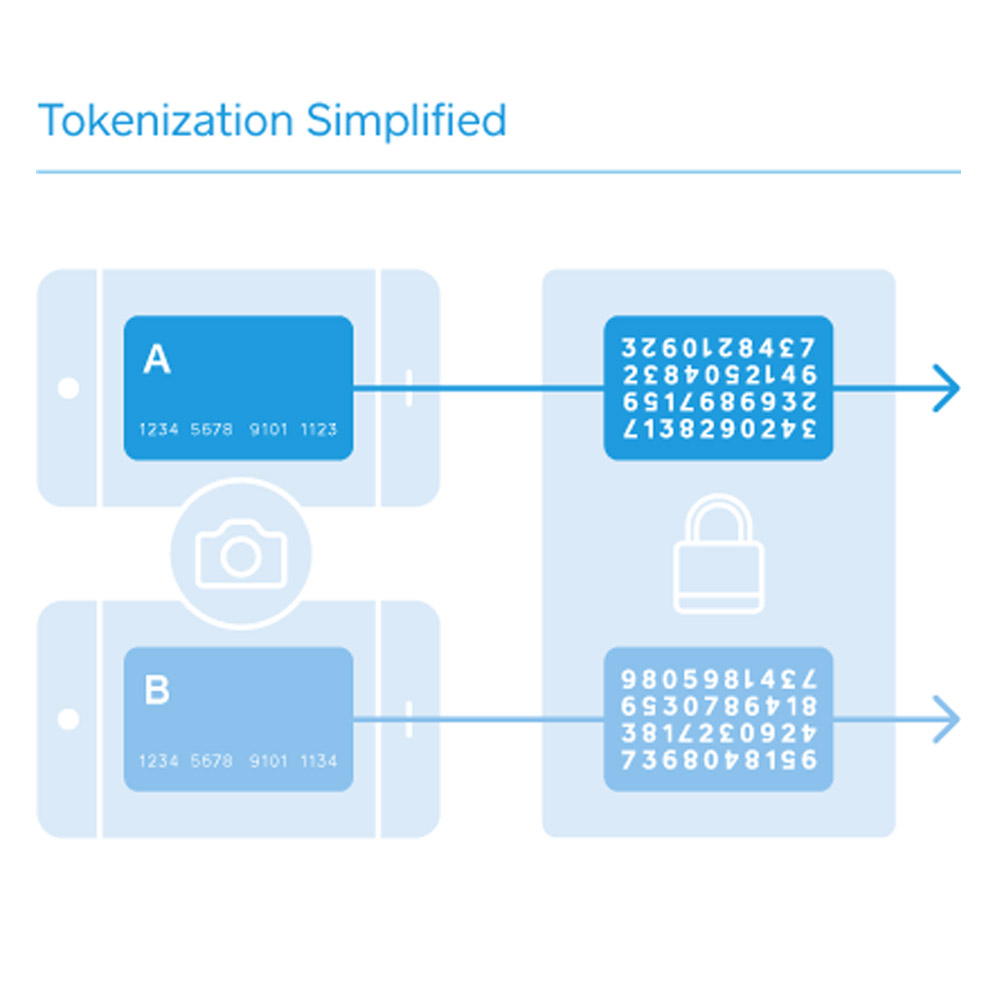
\includegraphics[scale=0.4]{figures/Chapter 7/1164067/Teori/Chapter7AnnisaFathoroni1.jpg}
    \caption{Train Inputs 1 - Annisa Fathoroni}
    \label{Train Inputs 1 - Annisa Fathoroni}
    \end{figure}
\end{itemize}

\subsubsection{Soal No. 7}
Maksud dari fungsi d train inputs = d train inputs/np.amax(np.absolute, , dilengkapi dengan ilustrasi atau gambar.

\begin{itemize}
\item Ilustrasi Gambar :

    \begin{figure}[!hbtp]
    \centering
    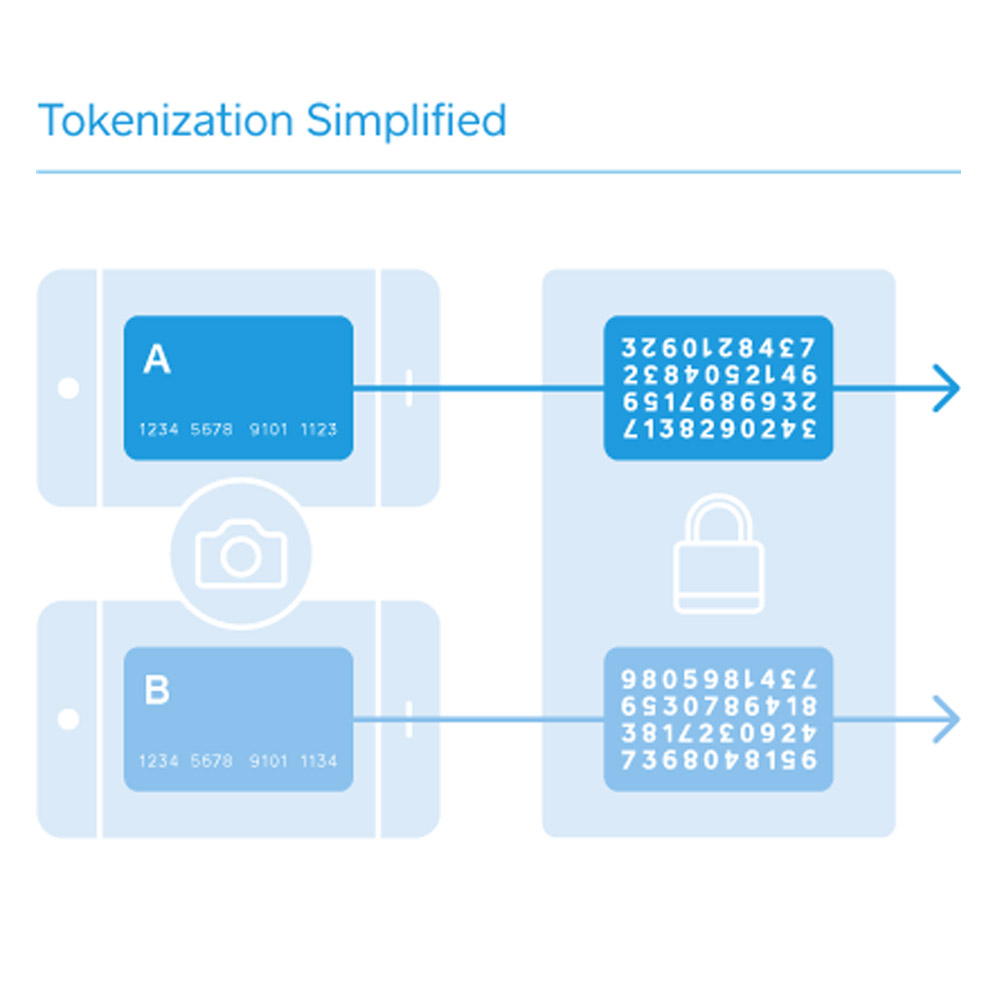
\includegraphics[scale=0.4]{figures/Chapter 7/1164067/Teori/Chapter7AnnisaFathoroni1.jpg}
    \caption{Train Inputs 2 - Annisa Fathoroni}
    \label{Train Inputs 2 - Annisa Fathoroni}
    \end{figure}
\end{itemize}

\subsubsection{Soal No. 10}
Maksud dari [caption=Compile model,label=lst:7.2] model.compile(loss=’categoricalcrossentropy0 , optimizer =0 adamax0 metrics = [0accuracy0])

\begin{itemize}
    \item Ilustrasi Gambar:

    \begin{figure}[!hbtp]
    \centering
    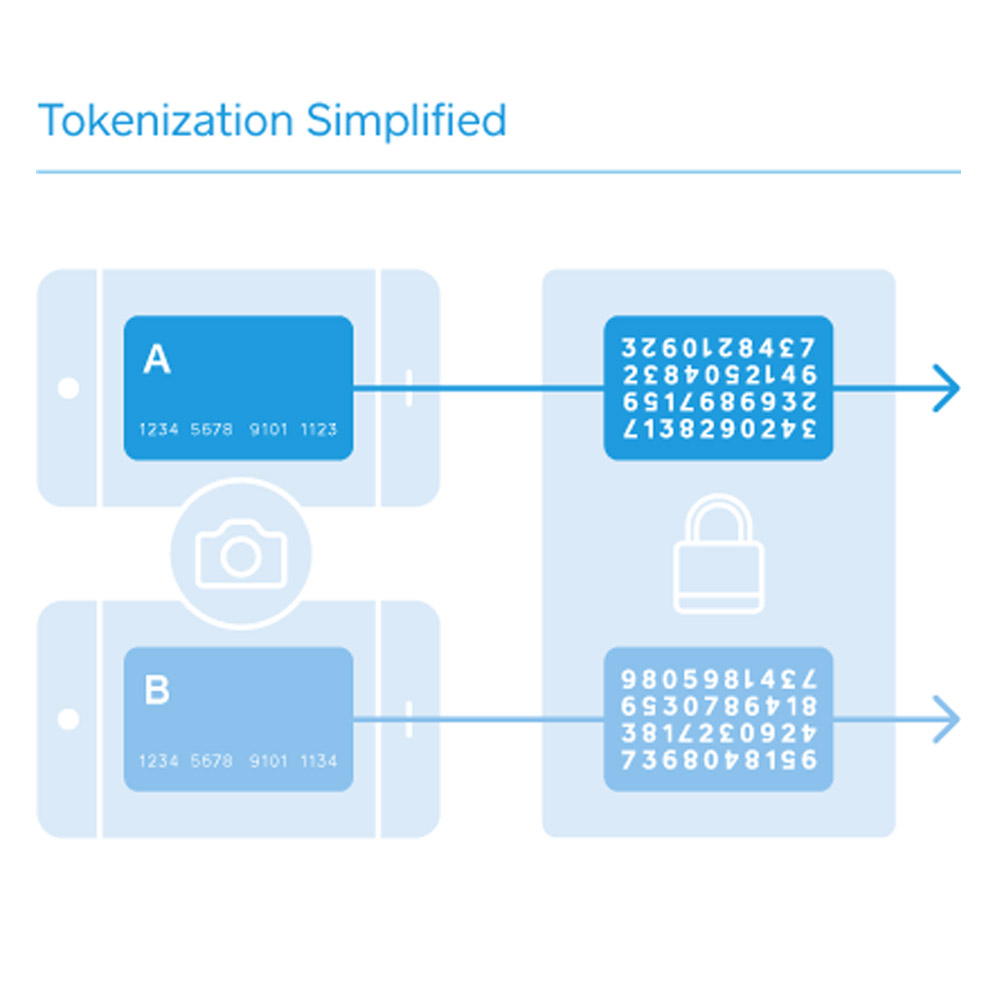
\includegraphics[scale=0.4]{figures/Chapter 7/1164067/Teori/Chapter7AnnisaFathoroni1.jpg}
    \caption{Compile model - Annisa Fathoroni}
    \label{Compile model - Annisa Fathoroni}
    \end{figure}
\end{itemize}

\subsubsection{Soal No. 11}
Deep Learning

\hfill \break
Deep learning, yang bisa diartikan sebagai rangkaian metode untuk melatih jaringan saraf buatan multi-lapisan. Ternyata, metode ini efektif dalam mengidentifikasi pola dari data. Manakala media membicarakan jaringan saraf, kemungkinan yang dimaksud adalah deep learning.

\subsubsection{Soal No. 12}
Deep Neural Network, dan apa bedanya dengan Deep Learning

\hfill \break
Algoritma DNN (Deep Neural Networks) adalah salah satu algoritma berbasis jaringan saraf yang dapat digunakan untuk pengambilan keputusan. Contoh yang dibahas kali ini adalah mengenai penentuan penerimaan pengajuan kredit sepeda motor baru berdasarkan kelompok data yang sudah ada.

Pebedaannya dengan Deep Learning adalah terletak pada kedalaman model, deep learning adalah frasa yang digunakan untuk jaringan saraf yang kompleks.

\subsubsection{Soal No. 13}
Jelaskan dengan ilustrasi gambar buatan sendiri, bagaimana perhitungan algoritma konvolusi dengan ukuran stride (NPM mod3+1)x(NPM mod3+1) yang terdapat max pooling.(nilai 30)

\begin{itemize}
    \item Ilustrasi Gambar:

    \begin{figure}[!hbtp]
    \centering
    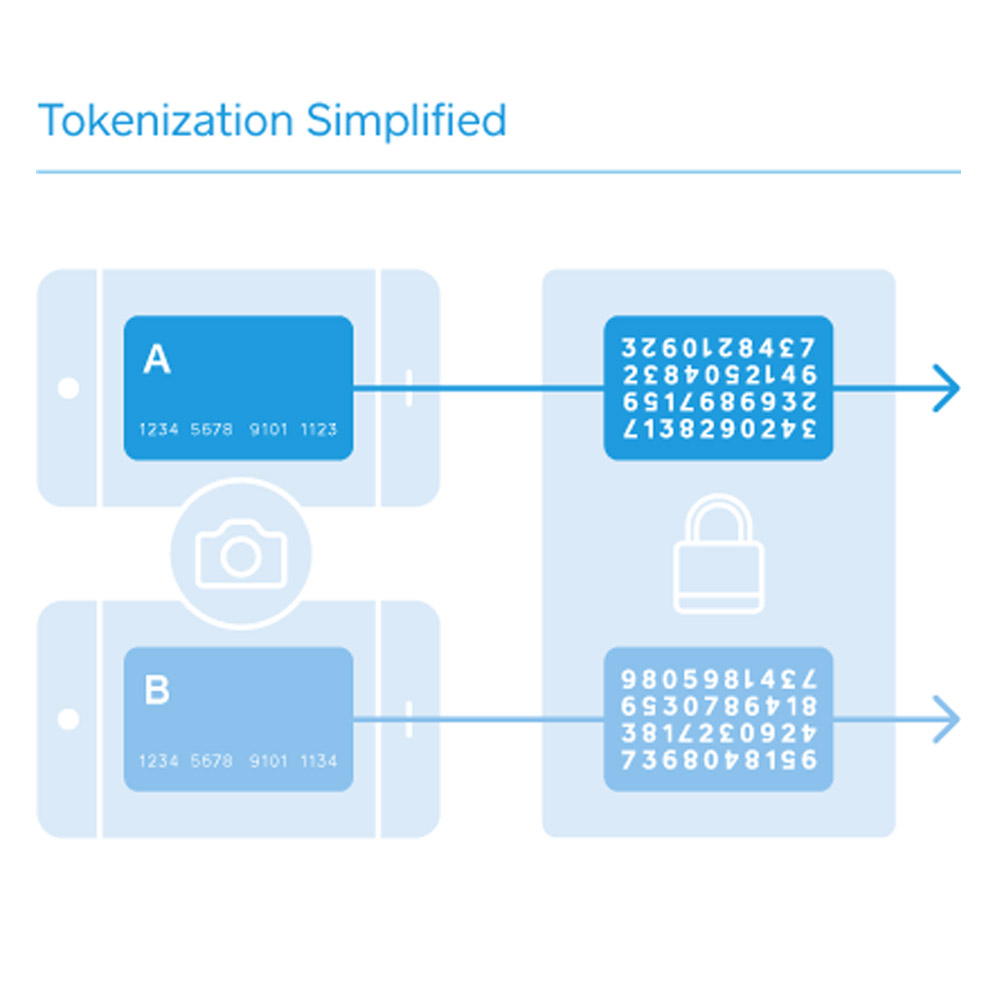
\includegraphics[scale=0.4]{figures/Chapter 7/1164067/Teori/Chapter7AnnisaFathoroni1.jpg}
    \caption{Perhitungan algoritma konvolusi - Annisa Fathoroni}
    \label{Perhitungan algoritma konvolusi - Annisa Fathoroni}
    \end{figure}
\end{itemize}

\subsection{Praktek}


\subsection{Penanganan Error}
